% Options for packages loaded elsewhere
\PassOptionsToPackage{unicode}{hyperref}
\PassOptionsToPackage{hyphens}{url}
%
\documentclass[
]{article}
\usepackage{amsmath,amssymb}
\usepackage{lmodern}
\usepackage{iftex}
\ifPDFTeX
  \usepackage[T1]{fontenc}
  \usepackage[utf8]{inputenc}
  \usepackage{textcomp} % provide euro and other symbols
\else % if luatex or xetex
  \usepackage{unicode-math}
  \defaultfontfeatures{Scale=MatchLowercase}
  \defaultfontfeatures[\rmfamily]{Ligatures=TeX,Scale=1}
\fi
% Use upquote if available, for straight quotes in verbatim environments
\IfFileExists{upquote.sty}{\usepackage{upquote}}{}
\IfFileExists{microtype.sty}{% use microtype if available
  \usepackage[]{microtype}
  \UseMicrotypeSet[protrusion]{basicmath} % disable protrusion for tt fonts
}{}
\makeatletter
\@ifundefined{KOMAClassName}{% if non-KOMA class
  \IfFileExists{parskip.sty}{%
    \usepackage{parskip}
  }{% else
    \setlength{\parindent}{0pt}
    \setlength{\parskip}{6pt plus 2pt minus 1pt}}
}{% if KOMA class
  \KOMAoptions{parskip=half}}
\makeatother
\usepackage{xcolor}
\IfFileExists{xurl.sty}{\usepackage{xurl}}{} % add URL line breaks if available
\IfFileExists{bookmark.sty}{\usepackage{bookmark}}{\usepackage{hyperref}}
\hypersetup{
  pdftitle={ANOVA},
  pdfauthor={Alan T. Arnholt},
  hidelinks,
  pdfcreator={LaTeX via pandoc}}
\urlstyle{same} % disable monospaced font for URLs
\usepackage[margin=1in]{geometry}
\usepackage{color}
\usepackage{fancyvrb}
\newcommand{\VerbBar}{|}
\newcommand{\VERB}{\Verb[commandchars=\\\{\}]}
\DefineVerbatimEnvironment{Highlighting}{Verbatim}{commandchars=\\\{\}}
% Add ',fontsize=\small' for more characters per line
\usepackage{framed}
\definecolor{shadecolor}{RGB}{248,248,248}
\newenvironment{Shaded}{\begin{snugshade}}{\end{snugshade}}
\newcommand{\AlertTok}[1]{\textcolor[rgb]{0.94,0.16,0.16}{#1}}
\newcommand{\AnnotationTok}[1]{\textcolor[rgb]{0.56,0.35,0.01}{\textbf{\textit{#1}}}}
\newcommand{\AttributeTok}[1]{\textcolor[rgb]{0.77,0.63,0.00}{#1}}
\newcommand{\BaseNTok}[1]{\textcolor[rgb]{0.00,0.00,0.81}{#1}}
\newcommand{\BuiltInTok}[1]{#1}
\newcommand{\CharTok}[1]{\textcolor[rgb]{0.31,0.60,0.02}{#1}}
\newcommand{\CommentTok}[1]{\textcolor[rgb]{0.56,0.35,0.01}{\textit{#1}}}
\newcommand{\CommentVarTok}[1]{\textcolor[rgb]{0.56,0.35,0.01}{\textbf{\textit{#1}}}}
\newcommand{\ConstantTok}[1]{\textcolor[rgb]{0.00,0.00,0.00}{#1}}
\newcommand{\ControlFlowTok}[1]{\textcolor[rgb]{0.13,0.29,0.53}{\textbf{#1}}}
\newcommand{\DataTypeTok}[1]{\textcolor[rgb]{0.13,0.29,0.53}{#1}}
\newcommand{\DecValTok}[1]{\textcolor[rgb]{0.00,0.00,0.81}{#1}}
\newcommand{\DocumentationTok}[1]{\textcolor[rgb]{0.56,0.35,0.01}{\textbf{\textit{#1}}}}
\newcommand{\ErrorTok}[1]{\textcolor[rgb]{0.64,0.00,0.00}{\textbf{#1}}}
\newcommand{\ExtensionTok}[1]{#1}
\newcommand{\FloatTok}[1]{\textcolor[rgb]{0.00,0.00,0.81}{#1}}
\newcommand{\FunctionTok}[1]{\textcolor[rgb]{0.00,0.00,0.00}{#1}}
\newcommand{\ImportTok}[1]{#1}
\newcommand{\InformationTok}[1]{\textcolor[rgb]{0.56,0.35,0.01}{\textbf{\textit{#1}}}}
\newcommand{\KeywordTok}[1]{\textcolor[rgb]{0.13,0.29,0.53}{\textbf{#1}}}
\newcommand{\NormalTok}[1]{#1}
\newcommand{\OperatorTok}[1]{\textcolor[rgb]{0.81,0.36,0.00}{\textbf{#1}}}
\newcommand{\OtherTok}[1]{\textcolor[rgb]{0.56,0.35,0.01}{#1}}
\newcommand{\PreprocessorTok}[1]{\textcolor[rgb]{0.56,0.35,0.01}{\textit{#1}}}
\newcommand{\RegionMarkerTok}[1]{#1}
\newcommand{\SpecialCharTok}[1]{\textcolor[rgb]{0.00,0.00,0.00}{#1}}
\newcommand{\SpecialStringTok}[1]{\textcolor[rgb]{0.31,0.60,0.02}{#1}}
\newcommand{\StringTok}[1]{\textcolor[rgb]{0.31,0.60,0.02}{#1}}
\newcommand{\VariableTok}[1]{\textcolor[rgb]{0.00,0.00,0.00}{#1}}
\newcommand{\VerbatimStringTok}[1]{\textcolor[rgb]{0.31,0.60,0.02}{#1}}
\newcommand{\WarningTok}[1]{\textcolor[rgb]{0.56,0.35,0.01}{\textbf{\textit{#1}}}}
\usepackage{longtable,booktabs,array}
\usepackage{calc} % for calculating minipage widths
% Correct order of tables after \paragraph or \subparagraph
\usepackage{etoolbox}
\makeatletter
\patchcmd\longtable{\par}{\if@noskipsec\mbox{}\fi\par}{}{}
\makeatother
% Allow footnotes in longtable head/foot
\IfFileExists{footnotehyper.sty}{\usepackage{footnotehyper}}{\usepackage{footnote}}
\makesavenoteenv{longtable}
\usepackage{graphicx}
\makeatletter
\def\maxwidth{\ifdim\Gin@nat@width>\linewidth\linewidth\else\Gin@nat@width\fi}
\def\maxheight{\ifdim\Gin@nat@height>\textheight\textheight\else\Gin@nat@height\fi}
\makeatother
% Scale images if necessary, so that they will not overflow the page
% margins by default, and it is still possible to overwrite the defaults
% using explicit options in \includegraphics[width, height, ...]{}
\setkeys{Gin}{width=\maxwidth,height=\maxheight,keepaspectratio}
% Set default figure placement to htbp
\makeatletter
\def\fps@figure{htbp}
\makeatother
\setlength{\emergencystretch}{3em} % prevent overfull lines
\providecommand{\tightlist}{%
  \setlength{\itemsep}{0pt}\setlength{\parskip}{0pt}}
\setcounter{secnumdepth}{5}
\ifLuaTeX
  \usepackage{selnolig}  % disable illegal ligatures
\fi

\title{ANOVA}
\author{Alan T. Arnholt}
\date{Last compiled: May 10, 2022 at 09:37:59 AM}

\begin{document}
\maketitle

{
\setcounter{tocdepth}{2}
\tableofcontents
}
\hypertarget{chapter-25-notes}{%
\section*{Chapter 25 Notes}\label{chapter-25-notes}}
\addcontentsline{toc}{section}{Chapter 25 Notes}

\textbf{Objectives:}

\begin{itemize}
\item
  Overview of ANOVA
\item
  Mathematics of ANOVA
\item
  Assumptions of ANOVA
\end{itemize}

\begin{center}\rule{0.5\linewidth}{0.5pt}\end{center}

The idea behind analysis of variance is to find out where the variance in the data lives. We have two possible estimates for the standard deviation of the errors. One is based on the standard deviation of the data differences from the group means, and one is based on the differences of the group means from the overall mean. We compare the differences between the means of the groups (\(SS_{\text{Between = Treatment}}\)) with the variation within the groups (\(SS_\text{Error = Residual = Within}\)).

\textbf{When the differences between means are large compared to the variation within the groups, we reject the null hypothesis and conclude the means are not all equal.}

\emph{The first step in analysis of variance problems is to make a comparative boxplot.}

We write our model as \(y_{ij}=\mu+\tau_i+\varepsilon_{ij}\), where \(\mu\) is the overall mean, \(\tau_i\) are the treatment effects, and \(\varepsilon_{ij}\) are the errors.

If the null hypothesis of all group means are equal, which is equivalent to \(H_0: \tau_1=\tau_2=\dots=\tau_k=0\), is true, the differences of the group means from the overall mean will be small compared to the differences of the data from the group means.

To estimate each of the parameters in our model, we use what you would expect:
\[\begin{array}{ccc}
\text{Parameter}&\text{Estimate}&\text{Name}\\
\mu&\bar{\bar{y}}&\text{Grand Mean}\\
\tau_i&\bar{y}_i - \bar{\bar{y}}&\text{Treatment Effect} (k \text{ of these})\\
\varepsilon_{ij}&y_{ij}-\bar{y}_i&\text{Residual}
\end{array}
\]

Consider the identity
\begin{equation}
y_{ij} - \bar{\bar{y}} = (\bar{y}_i - \bar{\bar{y}}) + (y_{ij} -
\bar{y}_i)
\label{eq:IDEN}
\end{equation}
which partitions the deviation of any observation from the grand mean into two parts. The first part, \((\bar{y}_i - \bar{\bar{y}})\), is the deviation of the \(i^{th}\) treatment mean from the grand mean. The second part is the deviation of the observation from the \(i^{th}\) treatment mean.

If all of the \(n_i\) values are the same, we have a balanced design\ldots which makes the calculation easier.

Squaring and summing both sides of \eqref{eq:IDEN} produces
\begin{align}
\sum_{i=1}^{k} \sum_{j=1}^{n_i} (y_{ij} - \bar{\bar{y}})^2 &=
\sum_{i=1}^{k} \sum_{j=1}^{n_i} \bigl[ (\bar{y}_i -
\bar{\bar{y}}) + (y_{ij} - \bar{y}_i)\bigr]^2\nonumber\\
&= \sum_{i=1}^k n_i (\bar{y}_i -
\bar{\bar{y}})^2 + \sum_{i=1}^{k} \sum_{j=1}^{n_i} (y_{ij} - \bar{y}_i)^2 \nonumber\\
&\quad+ 2 \sum_{i=1}^{k} \sum_{j=1}^{n_i} (\bar{y}_i -
\bar{\bar{y}})(y_{ij} - \bar{y}_i)
\label{eq:IDENA}
\end{align}
However, the cross product in \eqref{eq:IDENA} is zero since
\begin{equation*}
\sum_{j=1}^{n_i} (y_{ij} - \bar{y}_i) = \sum_{j=1}^{n_i} y_{ij} - n_i\bar{y}_i =
\sum_{j=1}^{n_i} y_{ij} - n_i \cdot \frac{\sum_{j=1}^{n_i} y_{ij}}{n_i} = 0.
\end{equation*}

\begin{center}\rule{0.5\linewidth}{0.5pt}\end{center}

After lots of algebra, we can derive the expression
\begin{equation}
\sum_{i=1}^{k} \sum_{j=1}^{n_i} (y_{ij} - \bar{\bar{y}})^2 =\sum_{i=1}^k
n_i (\bar{y}_i - \bar{\bar{y}})^2 + \sum_{i=1}^{k} \sum_{j=1}^{n_i}
(y_{ij} - \bar{y}_i)^2
\label{eq:SSIDEN}
\end{equation}
which says the total variability in the data can be partitioned into two parts. The quantity \(\sum_{i=1}^k n_i (\bar{y}_i - \bar{\bar{y}})^2\) measures the difference between the observed treatment means and the grand mean. Specifically, it is a measure of variability due to the treatments and is denoted \(SS_\text{Treatment}\) (sum of squares due to treatments). The quantity \(\sum_{i=1}^{k} \sum_{j=1}^{n_i} (y_{ij} - \bar{y}_i)^2\) measures the differences of observations within a treatment from the treatment mean, which must be due to error and is referred to as \(SS_\text{Error}\) (sum of squares due to error). The quantity on the left-hand side of the equals sign in \eqref{eq:SSIDEN} is called the total sum of squares corrected for the mean and is denoted \(SS_\text{Total}\). The symbolic representation of \eqref{eq:SSIDEN} is

\begin{equation}
SS_\text{Total} = SS_\text{Treatment} + SS_\text{Error}
\end{equation}

Since there are a total of \(\sum_{i=1}^k n_i= N\) observations, \(SS_\text{Total}\) has \(N-1\) degrees of freedom. One degree of freedom is lost for estimating \(\mu\) with the grand mean, \(\bar{\bar{y}}\).

\(SS_\text{Treatment}\) has \(k-1\) degrees of freedom since there are \(k\) treatment means and \(SS_\text{Error}\) has \(N-k\) degrees of freedom.

\begin{center}\rule{0.5\linewidth}{0.5pt}\end{center}

To adjust for the number of treatments, \(SS_\text{Treatment}\) is divided by its degrees of freedom, \(k-1\). The
resulting quantity is known as the \textbf{mean square treatment} \(MS_\text{Treatment} = \frac{SS_{\text{Treatment}}}{df_\text{Treatment}}\) and is also called the \textbf{between treatments error variance}.

In order to know whether the \(MS_\text{Treatment}\) value is large, it is compared to an estimate of \(\sigma^2\), namely, \(MS_\text{Error}\), where \(MS_\text{Error} = \frac{SS_{Error}}{df_{Error}}\), which is also called the \textbf{within treatments error variance.}

Note that \(MS_\text{Error}\) can be expressed as
\begin{equation}\label{MSerrorEQ}
\hat\sigma^2 = MS_\text{Error} = \frac{SS_{Error}}{df_{Error}} =
\frac{\sum_{i=1}^k \left[ \sum_{j=1}^{n_i} (y_{ij} - \bar{y}_i
)^2\right]}{df_\text{Error}}
\end{equation}

If the term within the square braces is divided by its degrees of freedom
\((n_i-1)\), it is easy to recognize that quantity as the sample variance for the
\(i^{th}\) treatment:\index{degrees of freedom}

\begin{equation}\label{sampvarithEQ}
S^2_i = \sum_{j=1}^{n_i} \frac{(y_{ij} - \bar{y}_i)^2}{n_i-1}, \: i=1,  2,  \dots, a
\end{equation}

Combining the sample variances, a single estimate of the population variance emerges as
\begin{align*}
\frac{(n_1-1) S^2_1 +(n_2-1)S^2_2+ \dots + (n_k-1)S^2_a}{(n_1-1) +(n_2-1)+
\dots + (n_k-1)} &= \frac{\sum_{i=1}^k \left[ \sum_{j=1}^{n_i} (y_{ij} -
\bar{y}_i)^2 \right]}{\sum_{i=1}^k (n_i-1)}\\
&= \frac{SS_\text{Error}}{N-k} = MS_\text{Error}
\end{align*}

The pooled estimate of the variance from the two-sample \(t\)-test has now been generalized for \(k\) different samples.

\begin{center}\rule{0.5\linewidth}{0.5pt}\end{center}

If there are no differences among the \(k\) treatment means, \(MS_\text{Treatment}\) is an unbiased estimate of \(\sigma^2\), and the ratio of \(MS_\text{Treatment}/MS_\text{Error}\) will be close to 1. If differences actually exist among the \(k\) treatment means, then the ratio, \(MS_\text{Treatment}/MS_\text{Error}\) should be larger than 1. In fact, it can be shown that

\begin{equation*}
E(MS_\text{Error}) = \sigma^2 \quad \text{ and }\quad E(MS_\text{Treatment})
= \sigma^2 + \sum_{i=1}^{k} \frac{n_i \tau_i^2}{k-1}
\end{equation*}

implying that when \(H_0\) is false, \(E(MS_\text{Treatment}) > E(MS_\text{Error})\) since some \(\tau_i\ne 0\). When \(H_0\) is true, \(\tau_i = 0 \, \text{ for all } i\) and \(E(MS_\text{Treatment}) = E(MS_\text{Error}) =\sigma^2\). With a little effort, it can be shown that

\begin{equation*}
\frac{MS_\text{Error}}{\sigma^2} \sim
\frac{\chi^2_{df_\text{Error}}}{df_\text{Error}} = \frac{\chi^2_{N-k}}{N-k}
\end{equation*}

regardless of whether \(H_0\) is true or not, and that

\begin{equation*}
\frac{MS_\text{Treatment}}{\sigma^2} \sim
\frac{\chi^2_{df_\text{Treatment}}}{df_\text{Treatment}} =
\frac{\chi^2_{k-1}}{k-1}
\end{equation*}

when \(H_0\) is true independently of \(MS_\text{Error}\).

\begin{center}\rule{0.5\linewidth}{0.5pt}\end{center}

When \(H_0\) is true, \(MSE\) and \(MST\) are similar, so the ratio is close to 1. If \(H_0\) is false, \(MS_T\) will be larger than \(MS_E\).

The sampling distribution of \(MS_\text{Treatment}/MS_\text{Error} \sim F_{k-1;\, N-k}\).

Thus, \(H_0\) is
rejected in an \(\alpha\)-level test if \(F_\text{obs} > f_{1-\alpha;\, k-1,\, N-k }\), where \(F_\text{obs} = MS_\text{Treatment}/MS_\text{Error}\).

In general, big \(F\)-statistics usually imply small p-values.

\begin{center}\rule{0.5\linewidth}{0.5pt}\end{center}

\textbf{Assumptions} To do an analysis of variance successfully, the assumptions must be met.

\begin{enumerate}
\def\labelenumi{\arabic{enumi}.}
\item
  Independence --- \(\checkmark\) Randomization

  \begin{itemize}
  \tightlist
  \item
    Surveys --- each group is representative
  \item
    Experiments --- subjects randomly assigned to groups and/or treatments
  \end{itemize}
\item
  Equal variance of treatment groups. Check similar spread of side-by-side boxplots of residuals \(y_{ij} - \bar{y}_i\) If the spread changes, consider \(\log y = y_{\star}\) in experiments, \(\sqrt{y}=y_{\star}\) in observational studies
\item
  Normal Population --- check for outliers in any group
\end{enumerate}

\hypertarget{example}{%
\subsection*{Example}\label{example}}
\addcontentsline{toc}{subsection}{Example}

Of the 23 first year male students at State U. admitted from Jim Thorpe High School, 8 were offered baseball scholarships and 7 were offered football scholarships. The University admissions committee looked at the students composite ACT scores (shown in the table), wondering if the University was lowering their standards for athletes. Assuming that this group of students is representative of all admitted students, what do you think?

\begin{Shaded}
\begin{Highlighting}[]
\NormalTok{Baseball }\OtherTok{\textless{}{-}} \FunctionTok{c}\NormalTok{(}\DecValTok{25}\NormalTok{, }\DecValTok{22}\NormalTok{, }\DecValTok{19}\NormalTok{, }\DecValTok{25}\NormalTok{, }\DecValTok{24}\NormalTok{, }\DecValTok{25}\NormalTok{, }\DecValTok{24}\NormalTok{, }\DecValTok{23}\NormalTok{)}
\NormalTok{NonAthlete }\OtherTok{\textless{}{-}} \FunctionTok{c}\NormalTok{(}\DecValTok{21}\NormalTok{, }\DecValTok{27}\NormalTok{, }\DecValTok{29}\NormalTok{, }\DecValTok{26}\NormalTok{, }\DecValTok{30}\NormalTok{, }\DecValTok{27}\NormalTok{, }\DecValTok{26}\NormalTok{, }\DecValTok{23}\NormalTok{)}
\NormalTok{Football }\OtherTok{\textless{}{-}} \FunctionTok{c}\NormalTok{(}\DecValTok{22}\NormalTok{, }\DecValTok{21}\NormalTok{, }\DecValTok{24}\NormalTok{, }\DecValTok{27}\NormalTok{, }\DecValTok{19}\NormalTok{, }\DecValTok{23}\NormalTok{, }\DecValTok{17}\NormalTok{)}
\NormalTok{DF }\OtherTok{\textless{}{-}} \FunctionTok{data.frame}\NormalTok{(}\AttributeTok{Score =} \FunctionTok{c}\NormalTok{(Baseball, NonAthlete, Football), }
                 \AttributeTok{Sport =} \FunctionTok{c}\NormalTok{(}\FunctionTok{rep}\NormalTok{(}\StringTok{"Baseball"}\NormalTok{, }\DecValTok{8}\NormalTok{), }\FunctionTok{rep}\NormalTok{(}\StringTok{"NonAthlete"}\NormalTok{, }\DecValTok{8}\NormalTok{), }
                           \FunctionTok{rep}\NormalTok{(}\StringTok{"Football"}\NormalTok{, }\DecValTok{7}\NormalTok{)))}
\NormalTok{GM }\OtherTok{\textless{}{-}} \FunctionTok{mean}\NormalTok{(DF}\SpecialCharTok{$}\NormalTok{Score)}
\NormalTok{GM}
\end{Highlighting}
\end{Shaded}

\begin{verbatim}
[1] 23.86957
\end{verbatim}

\begin{Shaded}
\begin{Highlighting}[]
\NormalTok{results }\OtherTok{\textless{}{-}}\NormalTok{ DF }\SpecialCharTok{\%\textgreater{}\%} 
  \FunctionTok{group\_by}\NormalTok{(Sport) }\SpecialCharTok{\%\textgreater{}\%} 
  \FunctionTok{summarize}\NormalTok{(}\FunctionTok{mean}\NormalTok{(Score), }\FunctionTok{sd}\NormalTok{(Score))}
\NormalTok{results}
\end{Highlighting}
\end{Shaded}

\begin{verbatim}
# A tibble: 3 x 3
  Sport      `mean(Score)` `sd(Score)`
  <fct>              <dbl>       <dbl>
1 Baseball            23.4        2.07
2 Football            21.9        3.29
3 NonAthlete          26.1        2.95
\end{verbatim}

\begin{Shaded}
\begin{Highlighting}[]
\CommentTok{\# Examine the data}
\FunctionTok{ggplot}\NormalTok{(}\AttributeTok{data =}\NormalTok{ DF, }\FunctionTok{aes}\NormalTok{(}\AttributeTok{x =}\NormalTok{ Sport, }\AttributeTok{y =}\NormalTok{ Score, }\AttributeTok{color =}\NormalTok{ Sport)) }\SpecialCharTok{+}
  \FunctionTok{geom\_hline}\NormalTok{(}\AttributeTok{yintercept =} \FunctionTok{c}\NormalTok{(}\FloatTok{23.86957}\NormalTok{, }\FloatTok{23.4}\NormalTok{, }\FloatTok{21.9}\NormalTok{, }\FloatTok{26.9}\NormalTok{), }
             \AttributeTok{color =} \FunctionTok{c}\NormalTok{(}\StringTok{"black"}\NormalTok{, }\StringTok{"red"}\NormalTok{, }\StringTok{"green"}\NormalTok{, }\StringTok{"blue"}\NormalTok{)) }\SpecialCharTok{+}
  \FunctionTok{geom\_boxplot}\NormalTok{() }\SpecialCharTok{+} 
  \FunctionTok{geom\_jitter}\NormalTok{(}\AttributeTok{width =} \FloatTok{0.2}\NormalTok{, }\AttributeTok{height =} \DecValTok{0}\NormalTok{) }\SpecialCharTok{+} 
  \FunctionTok{theme\_bw}\NormalTok{()}
\end{Highlighting}
\end{Shaded}

\begin{center}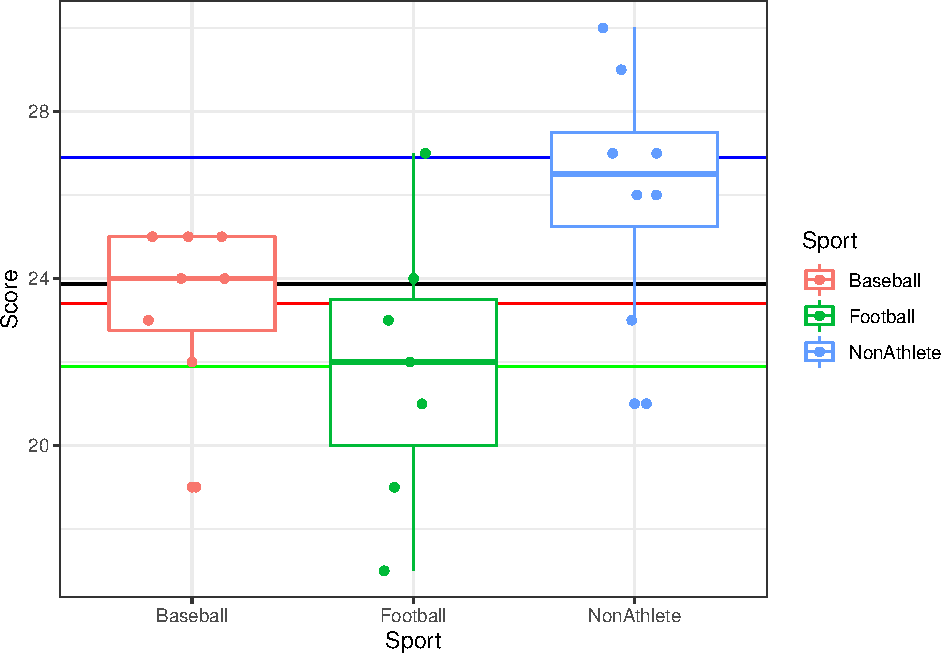
\includegraphics{SDM-CHAP25_files/figure-latex/unnamed-chunk-1-1} \end{center}

\begin{Shaded}
\begin{Highlighting}[]
\NormalTok{SSTreat }\OtherTok{\textless{}{-}} \DecValTok{8}\SpecialCharTok{*}\NormalTok{(}\FloatTok{23.375} \SpecialCharTok{{-}}\NormalTok{ GM)}\SpecialCharTok{\^{}}\DecValTok{2} \SpecialCharTok{+} \DecValTok{7}\SpecialCharTok{*}\NormalTok{(}\FloatTok{21.85714} \SpecialCharTok{{-}}\NormalTok{ GM)}\SpecialCharTok{\^{}}\DecValTok{2} \SpecialCharTok{+} \DecValTok{8}\SpecialCharTok{*}\NormalTok{(}\FloatTok{26.125} \SpecialCharTok{{-}}\NormalTok{ GM)}\SpecialCharTok{\^{}}\DecValTok{2}
\NormalTok{SSTreat}
\end{Highlighting}
\end{Shaded}

\begin{verbatim}
[1] 71.00163
\end{verbatim}

\begin{Shaded}
\begin{Highlighting}[]
\NormalTok{MSTreat }\OtherTok{\textless{}{-}}\NormalTok{ SSTreat}\SpecialCharTok{/}\DecValTok{2}
\NormalTok{MSTreat}
\end{Highlighting}
\end{Shaded}

\begin{verbatim}
[1] 35.50082
\end{verbatim}

\begin{Shaded}
\begin{Highlighting}[]
\NormalTok{SSError }\OtherTok{\textless{}{-}} \FunctionTok{sum}\NormalTok{((Baseball }\SpecialCharTok{{-}} \FloatTok{23.375}\NormalTok{)}\SpecialCharTok{\^{}}\DecValTok{2} \SpecialCharTok{+}\NormalTok{ (Football }\SpecialCharTok{{-}} \FloatTok{21.857143}\NormalTok{)}\SpecialCharTok{\^{}}\DecValTok{2} \SpecialCharTok{+}\NormalTok{ (NonAthlete }\SpecialCharTok{{-}} \FloatTok{26.125}\NormalTok{)}\SpecialCharTok{\^{}}\DecValTok{2}\NormalTok{)}
\NormalTok{SSError}
\end{Highlighting}
\end{Shaded}

\begin{verbatim}
[1] 155.6276
\end{verbatim}

\begin{Shaded}
\begin{Highlighting}[]
\NormalTok{MSError }\OtherTok{\textless{}{-}}\NormalTok{ SSError}\SpecialCharTok{/}\DecValTok{20}
\NormalTok{MSError}
\end{Highlighting}
\end{Shaded}

\begin{verbatim}
[1] 7.781378
\end{verbatim}

\begin{Shaded}
\begin{Highlighting}[]
\NormalTok{(F }\OtherTok{\textless{}{-}}\NormalTok{ MSTreat}\SpecialCharTok{/}\NormalTok{MSError)}
\end{Highlighting}
\end{Shaded}

\begin{verbatim}
[1] 4.562279
\end{verbatim}

\begin{Shaded}
\begin{Highlighting}[]
\NormalTok{(pvalue }\OtherTok{\textless{}{-}} \FunctionTok{pf}\NormalTok{(F, }\DecValTok{2}\NormalTok{, }\DecValTok{20}\NormalTok{, }\AttributeTok{lower =} \ConstantTok{FALSE}\NormalTok{))}
\end{Highlighting}
\end{Shaded}

\begin{verbatim}
[1] 0.02331881
\end{verbatim}

\begin{Shaded}
\begin{Highlighting}[]
\CommentTok{\#}
\FunctionTok{anova}\NormalTok{(}\FunctionTok{lm}\NormalTok{(Score }\SpecialCharTok{\textasciitilde{}}\NormalTok{ Sport, }\AttributeTok{data =}\NormalTok{ DF))}
\end{Highlighting}
\end{Shaded}

\begin{verbatim}
Analysis of Variance Table

Response: Score
          Df  Sum Sq Mean Sq F value  Pr(>F)  
Sport      2  71.002  35.501  4.5629 0.02331 *
Residuals 20 155.607   7.780                  
---
Signif. codes:  0 '***' 0.001 '**' 0.01 '*' 0.05 '.' 0.1 ' ' 1
\end{verbatim}

\textbf{There is evidence all the group means are not equal.}

Treat df = \# treatments \(-\, 1\)

Total df = \# treatments \(\times\) \# repetitions \(-\,1\).

Treat df + Error df = Total df, so Error df = Total df \(-\) Treat df.

In general the relationship between the tstat in a regular t-test and the F statistic is that \(t_\text{stat}^2 = F_\text{stat}\).

\begin{center}\rule{0.5\linewidth}{0.5pt}\end{center}

\textbf{Objectives:}

\begin{itemize}
\item
  Confidence interval and test for single comparison
\item
  CI for multiple comparisons
\item
  What can go wrong
\end{itemize}

\begin{center}\rule{0.5\linewidth}{0.5pt}\end{center}

To test \(H_0: \mu_1 - \mu_2 = 0\), we need:

\(SE(\bar{y}_1-\bar{y}_2) = s_p \sqrt{\dfrac{\strut 1}{n_1}+\dfrac{1}{n_2}}\) where \(s_p = \sqrt{MSE}= \sqrt{\dfrac{\sum_{i=1}^{k} \sum_{j=1}^{n_i} (y_{ij} - \bar{y}_i)^2}{N-k}}\), the pooled standard error from all the groups.

The \(t\)-test statistic is \(\dfrac{\bar{y}_1 - \bar{y}_2}{SE(\bar{y}_1-\bar{y}_2)}\), which will have \(N-k\) degrees of freedom and a \(t\) distribution.

If we wish to do multiple comparisons, we should use a critical value of \(t\) equal to \(t_{N-k; 1-\alpha/2\omega}\) where \(\omega\) is the number of pairs in the Bonferroni method. Other multiple comparison methods include Tukey, Dunn-Sidak, and Scheffe. \url{http://sci2s.ugr.es/keel/pdf/specific/articulo/35723.pdf} has a good explanation of several of the different multiple comparisons.

The \((1-\alpha)\cdot 100\%\) Bonferroni confidence interval for \(\mu_1-\mu_2\) is \(\bar{y}_1 - \bar{y}_2 \pm ME\) where the margin of error, \(ME= t_{N-k; 1-\alpha/2\omega} s_p \sqrt{\dfrac{\strut 1}{n_1}+\dfrac{1}{n_2}}\). Typically, you will evaluate computer output: if zero is in the CI, there is no evidence of a difference.

A Tukey CI is similar with \(ME = q(1-\alpha,r,df_\text{Error}) \cdot \sqrt{\dfrac{MS_\text{Error}}{2}\left( \dfrac{\strut 1}{n_1}+\dfrac{1}{n_2} \right)}\) where
\(q(1-\alpha,r,df_\text{Error})\) depends on the number of treatments and total number of data points, not on the individual treatments, so it's the same for all rows in any given experiment.

The command in R to look up values from a \(q\) distribution is \texttt{qtukey(q,\ nmeans\ =\ ,\ df\ =\ dferror)}. Where \texttt{q} is a vector of quantiles (area to the left\ldots{}\(1-\alpha_e\)).

Reference sites:

\begin{itemize}
\item
  \url{http://sci2s.ugr.es/keel/pdf/specific/articulo/35723.pdf}
\item
  \url{http://brownmath.com/stat/anova1.htm}
\end{itemize}

\begin{center}\rule{0.5\linewidth}{0.5pt}\end{center}

\textbf{Example}

Create Boxplots, check assumptions, perform ANOVA\ldots if significant\ldots perform Tukey posthoc comparisons.

\begin{Shaded}
\begin{Highlighting}[]
\NormalTok{TimeOfDay }\OtherTok{\textless{}{-}} \FunctionTok{c}\NormalTok{(}\FunctionTok{rep}\NormalTok{(}\StringTok{"Early\_7am"}\NormalTok{, }\DecValTok{16}\NormalTok{), }\FunctionTok{rep}\NormalTok{(}\StringTok{"Evening\_5pm"}\NormalTok{, }\DecValTok{16}\NormalTok{), }\FunctionTok{rep}\NormalTok{(}\StringTok{"LateEvening\_12am"}\NormalTok{, }\DecValTok{16}\NormalTok{))}
\NormalTok{TimeSeconds }\OtherTok{\textless{}{-}} \FunctionTok{c}\NormalTok{(}\DecValTok{68}\NormalTok{, }\DecValTok{138}\NormalTok{, }\DecValTok{75}\NormalTok{, }\DecValTok{186}\NormalTok{, }\DecValTok{68}\NormalTok{, }\DecValTok{217}\NormalTok{, }\DecValTok{93}\NormalTok{, }\DecValTok{90}\NormalTok{, }\DecValTok{71}\NormalTok{, }\DecValTok{154}\NormalTok{, }\DecValTok{166}\NormalTok{, }\DecValTok{130}\NormalTok{, }\DecValTok{72}\NormalTok{, }\DecValTok{81}\NormalTok{, }\DecValTok{76}\NormalTok{, }\DecValTok{129}\NormalTok{, }\DecValTok{299}\NormalTok{, }
                 \DecValTok{367}\NormalTok{, }\DecValTok{331}\NormalTok{, }\DecValTok{257}\NormalTok{, }\DecValTok{260}\NormalTok{, }\DecValTok{269}\NormalTok{, }\DecValTok{252}\NormalTok{, }\DecValTok{200}\NormalTok{, }\DecValTok{296}\NormalTok{, }\DecValTok{204}\NormalTok{, }\DecValTok{190}\NormalTok{, }\DecValTok{240}\NormalTok{, }\DecValTok{350}\NormalTok{, }\DecValTok{256}\NormalTok{, }\DecValTok{282}\NormalTok{, }\DecValTok{320}\NormalTok{, }
                 \DecValTok{216}\NormalTok{, }\DecValTok{175}\NormalTok{, }\DecValTok{274}\NormalTok{, }\DecValTok{171}\NormalTok{, }\DecValTok{187}\NormalTok{, }\DecValTok{213}\NormalTok{, }\DecValTok{139}\NormalTok{, }\DecValTok{139}\NormalTok{, }\DecValTok{226}\NormalTok{, }\DecValTok{128}\NormalTok{, }\DecValTok{236}\NormalTok{, }\DecValTok{128}\NormalTok{, }\DecValTok{217}\NormalTok{, }\DecValTok{196}\NormalTok{, }\DecValTok{201}\NormalTok{, }\DecValTok{161}\NormalTok{)}
\NormalTok{DF }\OtherTok{\textless{}{-}} \FunctionTok{data.frame}\NormalTok{(TimeOfDay, TimeSeconds)}
\FunctionTok{rm}\NormalTok{(}\StringTok{"TimeOfDay"}\NormalTok{, }\StringTok{"TimeSeconds"}\NormalTok{)}
\FunctionTok{library}\NormalTok{(tidyverse)}
\FunctionTok{ggplot}\NormalTok{(}\AttributeTok{data =}\NormalTok{ DF, }\FunctionTok{aes}\NormalTok{(}\AttributeTok{x =}\NormalTok{ TimeOfDay, }\AttributeTok{y =}\NormalTok{ TimeSeconds)) }\SpecialCharTok{+}
  \FunctionTok{geom\_boxplot}\NormalTok{() }\SpecialCharTok{+} 
  \FunctionTok{theme\_bw}\NormalTok{()}
\end{Highlighting}
\end{Shaded}

\begin{center}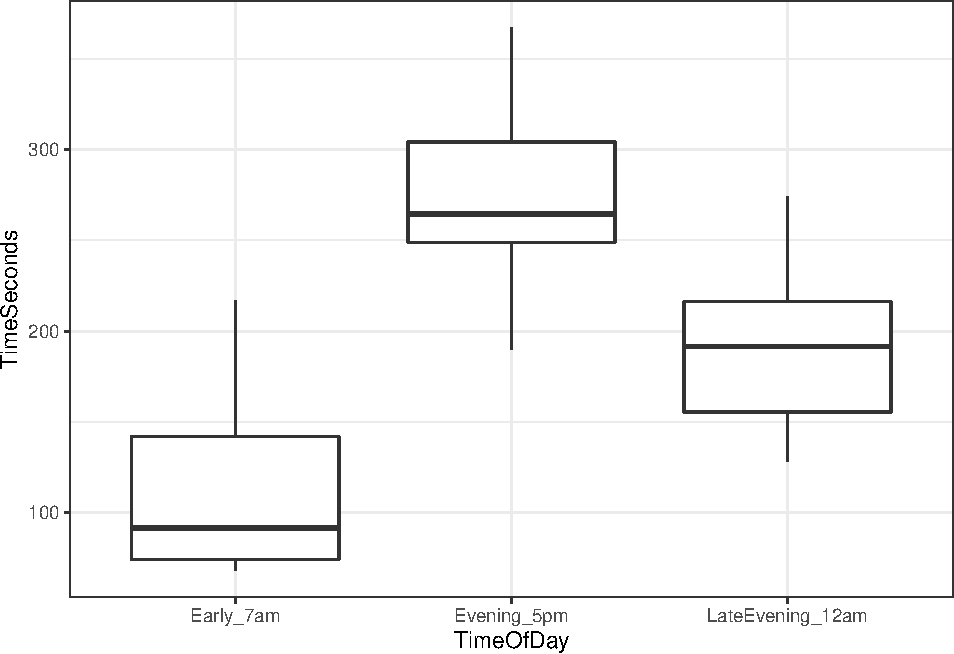
\includegraphics{SDM-CHAP25_files/figure-latex/unnamed-chunk-2-1} \end{center}

\begin{Shaded}
\begin{Highlighting}[]
\NormalTok{DF }\SpecialCharTok{\%\textgreater{}\%} 
  \FunctionTok{group\_by}\NormalTok{(TimeOfDay) }\SpecialCharTok{\%\textgreater{}\%} 
  \FunctionTok{summarize}\NormalTok{(}\FunctionTok{mean}\NormalTok{(TimeSeconds), }\FunctionTok{sd}\NormalTok{(TimeSeconds))}
\end{Highlighting}
\end{Shaded}

\begin{verbatim}
# A tibble: 3 x 3
  TimeOfDay        `mean(TimeSeconds)` `sd(TimeSeconds)`
  <fct>                          <dbl>             <dbl>
1 Early_7am                       113.              47.7
2 Evening_5pm                     273.              52.2
3 LateEvening_12am                188.              42.3
\end{verbatim}

\begin{Shaded}
\begin{Highlighting}[]
\FunctionTok{anova}\NormalTok{(}\FunctionTok{lm}\NormalTok{(TimeSeconds }\SpecialCharTok{\textasciitilde{}}\NormalTok{ TimeOfDay, }\AttributeTok{data =}\NormalTok{ DF))}
\end{Highlighting}
\end{Shaded}

\begin{verbatim}
Analysis of Variance Table

Response: TimeSeconds
          Df Sum Sq Mean Sq F value    Pr(>F)    
TimeOfDay  2 204952  102476  45.325 1.652e-11 ***
Residuals 45 101742    2261                      
---
Signif. codes:  0 '***' 0.001 '**' 0.01 '*' 0.05 '.' 0.1 ' ' 1
\end{verbatim}

\begin{Shaded}
\begin{Highlighting}[]
\FunctionTok{summary}\NormalTok{(mod }\OtherTok{\textless{}{-}} \FunctionTok{aov}\NormalTok{(TimeSeconds }\SpecialCharTok{\textasciitilde{}}\NormalTok{ TimeOfDay, }\AttributeTok{data =}\NormalTok{ DF))}
\end{Highlighting}
\end{Shaded}

\begin{verbatim}
            Df Sum Sq Mean Sq F value   Pr(>F)    
TimeOfDay    2 204952  102476   45.33 1.65e-11 ***
Residuals   45 101742    2261                     
---
Signif. codes:  0 '***' 0.001 '**' 0.01 '*' 0.05 '.' 0.1 ' ' 1
\end{verbatim}

\begin{Shaded}
\begin{Highlighting}[]
\FunctionTok{TukeyHSD}\NormalTok{(mod)}
\end{Highlighting}
\end{Shaded}

\begin{verbatim}
  Tukey multiple comparisons of means
    95% family-wise confidence level

Fit: aov(formula = TimeSeconds ~ TimeOfDay, data = DF)

$TimeOfDay
                                 diff        lwr       upr     p adj
Evening_5pm-Early_7am        159.9375  119.19361 200.68139 0.0000000
LateEvening_12am-Early_7am    74.5625   33.81861 115.30639 0.0001709
LateEvening_12am-Evening_5pm -85.3750 -126.11889 -44.63111 0.0000208
\end{verbatim}

\begin{Shaded}
\begin{Highlighting}[]
\FunctionTok{plot}\NormalTok{(}\FunctionTok{TukeyHSD}\NormalTok{(mod))}
\end{Highlighting}
\end{Shaded}

\begin{center}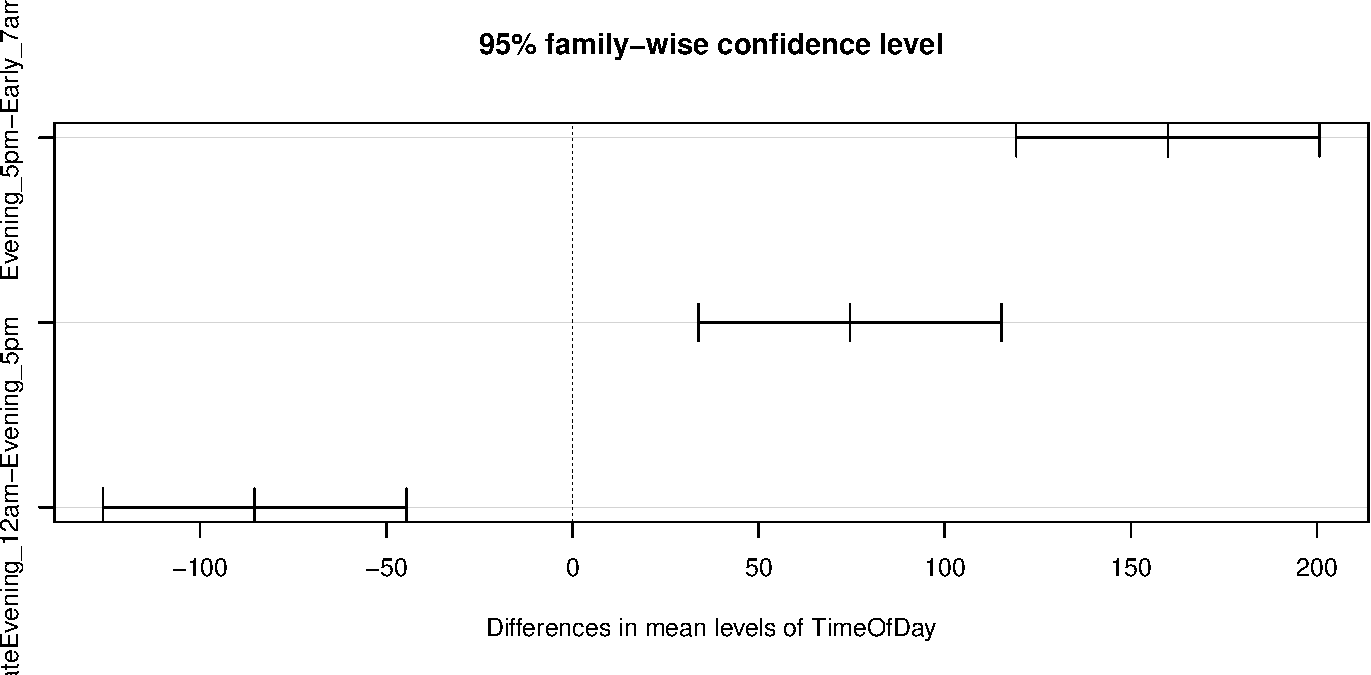
\includegraphics{SDM-CHAP25_files/figure-latex/unnamed-chunk-3-1} \end{center}

\end{document}
